\section{Tile-based Editor Calculus}\label{sec:formalism-2}

We now precisely characterize tile-based editing
as a calculus called \ty.
The punchline of \ty~ is the action judgment
$\performAction{\editState_1}{\action}{\editState_2}$,
which sends edit state $\editState_1$ to $\editState_2$
via action $\action$, and its governing invariant
that actions preserve parsability into a well-formed
program term.

We will begin our presentation in Section \ref{sec:zippers}
by describing the syntax of edit states $Z$.
Then, in Section \ref{sec:actions}, we will present each rule
defining the action judgment
$\performAction{\editState_1}{\action}{\editState_2}$,
describing supporting judgments and relevant metatheory
along the way.
% Our discussion will use concrete examples
% centered around edit states of the following program.
% \begin{center}
%   \texttt{\textbf{let} f = $\boldsymbol{\lambda}$ a , b \textbf{.} \textbf{(} a + b \textbf{)} / \textbf{(} a * b \textbf{)} \textbf{in} $\ophole$}
% \end{center}

\subsection{Zippers} \label{sec:zippers}

\begin{figure}
  \[\arraycolsep=3pt\begin{array}{rlrl}
      \text{zipper} & \zip & ::= & \zipper{\subject}{\zframe} \\
      \text{subject} & \subject & ::= &
        \pointing{\selection}{\selection} ~\vert~
        \selecting{\selection}{\selection}{\selection} ~\vert~
        \restructuring{\selection}{\selection}{\selection} \\
      \text{frame} & \zframe & ::= &
        \tfrelem^{\pat} ~\vert~ \tfrelem^{\expr}
 \end{array}\]
  \caption{
    Zipper syntax
  }
  \label{fig:zipper-syntax}
\end{figure}


Figure \ref{fig:zipper-syntax} shows the syntax of \ty~ edit states $\zip$,
which follow a variant of the well-known
\emph{zipper} pattern \cite{zipper}.
In particular, they have a \emph{bottom-up} zipper
structure---decomposing the total edit state $\zip$ into a
focused substructure $\subject$ and its surrounding context
$\zframe$---unlike the top-down structure used in other
work \cite{Hazelnut}.
In this work, we refer to $B$ as the \emph{subject} and $M$
as the \emph{frame}.

\paragraph{Subjects}
Subjects $\subject$ are modal, the three
variants corresponding to the pointing, selecting,
and restructuring modes we described using \tylr~
in Section \ref{sec:overview}.
Each mode decomposes the total subject into two
or three \emph{segments} $\selection$.
This decomposition encodes text-like cursor
placement between syntactic entities.
For example, consider the \tylr~ edit state
in pointing mode shown below;
\begin{center}
  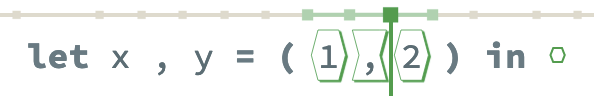
\includegraphics[width=\columnwidth]{img/zipper-example-1.png}
\end{center}
the corresponding subject in \ty~ is
$\pointing{\soptile{\svar{a}}}{\sbintile{\tplus}\soptile{\svar{b}}}$.

% \begin{figure}
% \centering
% \begin{subfigure}[c]{0.65\columnwidth}
%   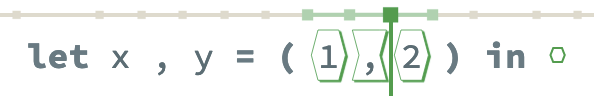
\includegraphics[width=\textwidth]{img/zipper-example-1.png}
%   \caption{}\label{fig:pointing-zipper-example}
% \end{subfigure}
% \begin{subfigure}[c]{0.65\columnwidth}
%   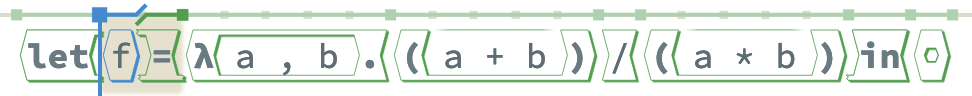
\includegraphics[width=\textwidth]{img/zipper-example-2.png}
%   \caption{}\label{fig:selecting-zipper-example}
% \end{subfigure}
% \caption{\note{todo}}
% \label{fig:zipper-examples}
% \end{figure}

\begin{figure}
\[\arraycolsep=3pt\begin{array}{rlrl}
  \text{segment} & \selection & ::= &
  \selem_1\dots\selem_n \\
  \text{piece} & \selem & ::= &
    \tile ~\vert~
    \shard \\

  \text{tile} & \tile & ::= &
      \tile^{\pat} ~\vert~
      \tile^{\expr} \\

  \text{shard} & \shard & ::= &
    \shard^{\pat} ~\vert~
    \shard^{\expr}
\end{array}\]
\caption{
  Syntax of segments
}
\label{fig:segment-syntax}
\end{figure}
\begin{figure}
  \[\arraycolsep=4pt\begin{array}{rlrl}
    \text{pattern shard} & \shard^{\pat} & ::= &
      \shardlit{\texttt{(}} ~\vert~
      \shardlit{\texttt{)}} \\
    \text{expression shard} & \shard^{\expr} & ::= &
      \shardlit{\texttt{(}} ~\vert~
      \shardlit{\texttt{)}} ~\vert~
      \shardlit{$\lambda$} ~\vert~
      \shardlit{\texttt{.}} ~\vert~
      \shardlit{\texttt{let}} ~\vert~
      \shardlit{\texttt{=}} ~\vert~
      \shardlit{\texttt{in}}
  \end{array}\]
  \caption{Syntax of pattern and expression shards}
  \label{fig:shard-syntax-2}
\end{figure}


Segments $\selection$ are sequences of \emph{tiles}
and \emph{shards}, collectively called \emph{pieces},
as shown in Figure \ref{fig:segment-syntax}.
Segments containing only tiles are called \emph{intact},
otherwise \emph{cracked}.
The two segments $\soptile{\svar{a}}$ and
$\sbintile{\tplus}\soptile{\svar{b}}$ in the last example consist
entirely of expression tiles $\tile^{\expr}$,
the syntax for which was given in Figure \ref{fig:tile-syntax}.
Meanwhile, the subject of the \tylr~ edit state shown below
\begin{center}
  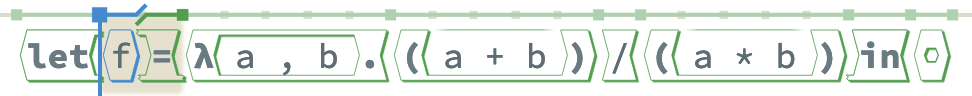
\includegraphics[width=\columnwidth]{img/zipper-example-2.png}
\end{center}
% \begin{figure}[h]
%   \centering
%   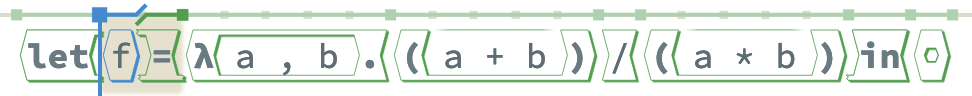
\includegraphics[width=0.65\columnwidth]{img/zipper-example-2.png}
% \end{figure}
is represented in \ty~ as
\newcommand{\lamab}{\spretile{\tlam{\sprod{\svar{a}}{\svar{b}}}}}
\newcommand{\parenaplusb}{\soptile{\sparen{\splus{\svar{a}}{\svar{b}}}}}
\newcommand{\parenamultb}{\soptile{\sparen{\smult{\svar{a}}{\svar{b}}}}}
\[
  \selecting{\shardlit{let}}{\soptile{\svar{f}}\shardlit{=}}{%
    \lamab
    \parenaplusb
    \sbintile{\tdiv}
    \parenamultb
    \shardlit{in}
    \soptile{\ophole}
  }.
\]
(We elide the grey-outline decorations on nested pieces
for visual clarity.)
% $\selecting{\shardlit{(}\soptile{\snumlit{1}}\sbintile{\tprod}}{\soptile{\snumlit{2}}\shardlit{)}}{\cdot}$.
In this case, the three segments making up the selecting subject each
contain an expression shard $\shard^{\expr}$,
the syntax for which is given in Figure \ref{fig:shard-syntax-2}.

\begin{figure}
  \vspace{-3px}
  \[
  \arraycolsep=3pt\begin{array}{rlrl}
      \mathsf{TilesFrame} & \tframe^s & ::= & \tframelit{\tiles^s\_\tiles^s}{\tfrelem^s} \\
      % \mathsf{Tile}^{\typ} & \tile^{\typ} & ::= &
      %     % \tnum ~\vert~
      %     \shole ~\vert~
      %     \sbool ~\vert~
      %     \snum ~\vert~
      %     \sarr{}{} ~\vert~
      %     \sprod{}{} ~\vert~
      %     \sparen{\tiles^{\typ}}\\
      \mathsf{PatTileFrame} & \tfrelem^{\pat} & ::= &
        \tframelit{\sparen{\_}}{\tframe^{\pat}} \\
      & & \vert &
        \tframelit{\slam{\_}{}}{\tframe^{\expr}} \\
      & & \vert &
        \tframelit{\slet{\_}{\tiles^{\expr}}{}}{\tframe^{\expr}} \\
      \mathsf{ExpTileFrame} & \tfrelem^{\expr} & ::= &
        \tframelit{\sparen{\_}}{\tframe^{\expr}} \\
      & & \vert &
        \tframelit{\slet{\tiles^{\pat}}{\_}{}}{\tframe^{\expr}}
        % \scond{}{\tiles^{\expr}}{}
  \end{array}\]
  \caption{
    Syntax of pattern and expression frames.
  }
  \label{fig:tile-syntax}
\end{figure}


\paragraph{Frames}
Frames model the rest of the edit state not included
in the subject.
At a high level, frames may be understood as a
list of nested containers,
arranged bottom-up such that the first container immediately
wraps the subject, each container other than the last points to its
parent container, and the last represents the edit state root.

Revisiting Figure \ref{fig:zipper-syntax},
frames $\zframe$ are sort-indexed \emph{tile frames}
$\tfrelem^s$, the syntax for which is given in Figure \ref{fig:frame-syntax}.
Tile frames $\tfrelem^s$ represent tiles with a missing
child of sort $s$.
Other than the program root $\froot$, we annotate tile frame literals
with $\framehole$ symbols in place of the missing child.
Each tile frame $\tfrelem^s$ additionally points to its parent
\emph{sequence frame} $\tframe^{s'}$, which carries the tile frame's
sibling tiles of sort $s'$ (possibly different from $s$).
Each sequence frame $\tframe^s$ in turn points to its parent
tile frame $\tfrelem^s$.
For example, the frames corresponding to the two
subject examples described earlier are, respectively,
\newcommand{\parenfrm}{\tframelit{\soptile{\sparen{\framehole}}}{\lamab\framehole\sbintile{\tdiv}\parenamultb}}
\newcommand{\letfrm}{\tframelit{\spretile{\tlet{\svar{f}}{\framehole}}}{\emptyseg\framehole\tophole}}
\begin{align*}
  & \parenfrm \\
  \tsframelit\ \ & \letfrm \\
  \tsframelit\ \ & \froot
\end{align*}
and $\froot$.
Moving forward, for brevity, we will elide $\tsframelit~\froot$ from the
end of non-root frames.

\paragraph{Cursor erasure}
Given a zipper $\zip$, we will often wish to refer to the
underlying segment $\erasezip{\zip}$ without regard for
how the cursor is positioned.
The operator $\erasezip{\cdot}$ is called \emph{cursor erasure}
and is defined for zippers below.
\[
  \erasezip{(\zipper{\subject}{\zframe})} = \fillFrame{\erasesub{\subject}}{\zframe}
\]
This definition depends on two sub-operations:
cursor erasure $\erasezip{\cdot}$ on subjects
and \emph{frame filling} $\fillFrame{\cdot}{\cdot}$.

Cursor erasure is defined for pointing subjects as follows.
\[\arraycolsep=2pt\begin{array}{rcl}
  \erasesub{(\pointing{\selection_1}{\selection_2})} & = & \selection_1\selection_2 \\
\end{array}\]
We will define cursor erasure on selecting and
restructuring subjects in Section \ref{sec:selecting}
after we have developed some additional machinery.

Frame filling $\fillFrame{\cdot}{\cdot}$, defined below,
takes a frame on the right and fills it with the segment
on the left to produce the total unfocused segment.
\[\begin{array}{cl}
  & \fillFrame{\tiles^{\expr}}{\froot}\ =\ \tiles^{\expr} \\\\

  & \fillFrame{\tiles^{s}}{
    \tframelit{
      \soptile{\sparen{\framehole}}
    }{
      \sframelit{\tiles_1^s\framehole\tiles_2^s}{\tfrelem^s}
    }
  } \\
  = &
    \fillFrame{
      \tiles_1^s\soptile{\sparen{\tiles^s}}\tiles_2^s
    }{\tfrelem^s} \\\\

  & \fillFrame{\tiles^{\pat}}{
    \tframelit{
      \spretile{\tlam{\framehole}}
    }{
      \sframelit{\tiles_1^\expr\framehole\tiles_2^\expr}{\tfrelem^\expr}
    }
  } \\
  = &
    \fillFrame{
      \tiles_1^\expr\spretile{\tlam{\tiles^\pat}}\tiles_2^\expr
    }{\tfrelem^\expr} \\\\

  & \fillFrame{\tiles^{\pat}}{
    \tframelit{
      \spretile{\tlet{\framehole}{\tiles^\expr}}
    }{
      \sframelit{\tiles_1^\expr\framehole\tiles_2^\expr}{\tfrelem^\expr}
    }
  } \\
  = &
    \fillFrame{
      \tiles_1^\expr\spretile{\tlet{\tiles^\pat}{\tiles^{\expr}}}\tiles_2^\expr
    }{\tfrelem^\expr} \\\\

  & \fillFrame{\tiles^{\expr}}{
    \tframelit{
      \spretile{\tlet{\tiles^\pat}{\framehole}}
    }{
      \sframelit{\tiles_1^\expr\framehole\tiles_2^\expr}{\tfrelem^\expr}
    }
  } \\
  = &
    \fillFrame{
      \tiles_1^\expr\spretile{\tlet{\tiles^\pat}{\tiles^{\expr}}}\tiles_2^\expr
    }{\tfrelem^\expr}
\end{array}\]
Note that frame filling is only partially defined for when the
left segment argument is a sequence of tiles of the
expected sort.
This implies that whenever cursor erasure succeeds on a zipper $\zipper{\subject}{\zframe}$,
then the cursor-erased subject $\erasesub{\subject}$ must be intact.

\subsection{Actions} \label{sec:actions}

\begin{figure}
  \vspace{-3px}
  \[
  \arraycolsep=3pt\begin{array}{rlrl}
      \mathsf{Action} & \action & ::= &
        \actionlit{mark} ~\vert~
        \actionlit{move}~\direction ~\vert~
        \actionlit{delete} ~\vert~
        \actionlit{construct}~\tile^s \\
      \mathsf{Direction} & \direction & ::= &
        \texttt{left} ~\vert~
        \texttt{right}
  \end{array}\]
  \caption{Syntax of actions}
  \label{fig:action-syntax}
\end{figure}


Figure \ref{fig:action-syntax} gives the syntax of actions $\action$.
Actions are given meaning by the action judgment
$\performAction{\editState_1}{\action}{\editState_2}$,
which we will define over the course of this section.
Moving forward, we will adopt the new notation $\termm^{\pat}$
and $\termm^{\expr}$ in place of $\spat$ and $\sexp$,
as were defined in Figure \ref{fig:term-syntax},
and $\termm^s$ for a term whose sort may vary.

\begin{figure}
  \judgbox{\flattenTerm{p}{\tiles^{\pat}}}{$p$ flattens to $\tiles^{\pat}$}
  \begin{mathpar}
    \inferrule[]{
    }{
      \flattenTerm{\term{\ophole}}{\optile{\ophole}}
    }\hspace{20pt}
    \inferrule[]{
    }{
      \flattenTerm{\term{\svar{x}}}{\optile{\svar{x}}}
    }\hspace{20pt}
    \inferrule[]{
      \flattenTerm{p}{\tiles^{\pat}}
    }{
      \flattenTerm{\term{\sparen{p}}}{\optile{\sparen{\tiles^{\pat}}}}
    }\\
    \inferrule[]{
      \flattenTerm{p_1}{\tiles^{\pat}_1} \\
      \flattenTerm{p_2}{\tiles^{\pat}_2}
    }{
      \flattenTerm{\term{\sbinhole{p_1}{p_2}}}{\tiles^{\pat}_1~\bintile{\binhole}~\tiles^{\pat}_2}
    }\hspace{20pt}
    \inferrule[]{
      \flattenTerm{p_1}{\tiles^{\pat}_1} \\
      \flattenTerm{p_2}{\tiles^{\pat}_2}
    }{
      \flattenTerm{\term{\sprod{p_1}{p_2}}}{\tiles^{\pat}_1~\bintile{\tprod}~\tiles^{\pat}_2}
    }
  \end{mathpar}

  \vspace{10pt}
  \judgbox{\flattenTerm{e}{\tiles^{\expr}}}{$e$ flattens to $\tiles^{\expr}$}
  \begin{mathpar}
    \inferrule[]{
    }{
      \flattenTerm{\term{\ophole}}{\optile{\ophole}}
    }\hspace{15pt}
    \inferrule[]{
    }{
      \flattenTerm{\term{\snumlit{n}}}{\optile{\snumlit{n}}}
    }\hspace{15pt}
    \inferrule[]{
    }{
      \flattenTerm{\term{\svar{x}}}{\optile{\svar{x}}}
    }\hspace{15pt}
    \inferrule[]{
      \flattenTerm{e}{\tiles^{\expr}}
    }{
      \flattenTerm{\term{\sparen{e}}}{\optile{\sparen{\tiles^{\expr}}}}
    }\\
    \inferrule[]{
      \flattenTerm{e_1}{\tiles^{\expr}_1} \\
      \flattenTerm{e_2}{\tiles^{\expr}_2}
    }{
      \flattenTerm{\term{\sbinhole{e_1}{e_2}}}{\tiles^{\expr}_1~\bintile{\binhole}~\tiles^{\expr}_2}
    }\hspace{20pt}
    \inferrule[]{
      \flattenTerm{e_1}{\tiles^{\expr}_1} \\
      \flattenTerm{e_2}{\tiles^{\expr}_2}
    }{
      \flattenTerm{\term{\sprod{e_1}{e_2}}}{\tiles^{\expr}_1~\bintile{\tprod}~\tiles^{\expr}_2}
    }\\
    \inferrule[]{
      \flattenTerm{p}{\tiles^{\pat}} \\
      \flattenTerm{e}{\tiles^{\expr}}
    }{
      \flattenTerm{\term{\slam{p}{e}}}{\pretile{\tlam{\tiles^{\pat}}}~\tiles^{\expr}}
    }\\
    \inferrule[]{
      \flattenTerm{p}{\tiles^{\pat}} \\
      \flattenTerm{e_1}{\tiles^{\expr}_1} \\
      \flattenTerm{e_2}{\tiles^{\expr}_2}
    }{
      \flattenTerm{\term{\slet{p}{e_1}{e_2}}}{\pretile{\tlet{\tiles^{\pat}}{\tiles^{\expr}_1}}~\tiles^{\expr}_2}
    }
  \end{mathpar}

  \caption{
    Term flattening
  }
  \label{fig:flatten-term}
  \end{figure}

We begin with the central \emph{parsability invariant}
governing the action judgment's design.
A segment $C$ is called \emph{$s$-parsable} if there
exists a term $\termm^s$ that \emph{flattens} to
it, as defined by the term flattening judgments $\flattenTerm{\termm^s}{C}$
given in Figure \ref{fig:flatten-term}.
Term flattening is akin to switching from term view
to tile view in \tylr, as we saw in Figure \ref{fig:pan}.
For example, the rules of term flattening would let us
derive the conclusion
\[
  \flattenTerm{
    \term{\slam{\sprod{a}{b}}{\sdiv{\sparen{\splus{\svar{a}}{\svar{b}}}}{\smult{\svar{a}}{\svar{b}}}}}
  }{
    \lamab
    \parenaplusb
    \sbintile{\tdiv}
    \parenamultb
  }.
\]
The parsability invariant is as follows.

\begin{theorem} \label{thm:parsability-invariant}
If $\erasezip{\zip_1}$ is $\expr$-parsable and $\performAction{\zip_1}{\action}{\zip_2}$
then $\erasezip{\zip_2}$ is $\expr$-parsable.
\end{theorem}

With this guideline in mind, we will now describe
each of the eight rules defining the action judgment,
grouped into five feature categories:
moving, % (\ref{sec:moving}),
inserting, % (\ref{sec:inserting}),
selecting, % (\ref{sec:selecting}),
restructuring, and % (\ref{sec:restructuring}), and
removing. % (\ref{sec:removing}).

While the action judgment is fully defined, the proofs of its
metatheory are in-progress;
in the meantime, we count \tylr's so-far-bug-free
experience as a small measure of empirical proof
of our approach.
The exposition in this section is incomplete as well,
petering out at the end of Section \ref{sec:inserting}, due
to lack of time.

% \note{introduce action syntax}

% \note{remark on first two rules taking the longest to establish setup,
% after which remaining six rules build on top of that}

% Our design of zipper operations diverges from prior art
% in our pursuit of linear text-like interactivity.
% Prior zipper designs are strictly hierarchical and ask
% the client to navigate in a structure-aware two-dimensional
% fashion: left and right to traverse siblings,
% up and down to traverse parent-child relations.
% In contrast, we aim to support a one-dimensional interaction
% model:
% it should be possible to navigate freely by moving solely
% left and right \note{might need to clarify or change wording
% here to address comparison with ordered traversals of trees};
% furthermore it should be possible to specify
% arbitrary subranges of a one-dimensional serialization
% of the total structure.
% Toward these ends, actions in \ty~ rely
% on a form of incremental unparsing and reparsing by which
% hierarchical structures may be ``flattened'' as needed
% to support linear traversal and partial selection.


\subsubsection{Moving} \label{sec:moving}

\ty's actions are designed around
a one-dimensional interaction model, where the client may
view the total edit state as its serialization, navigate through it
in a linear fashion, and select arbitrary subranges.
Toward these ends, actions rely
on a form of incremental unparsing and reparsing---distinct
from term flattening---by which
hierarchical structures may be temporarily serialized
as needed for linear traversal or partial selection.
In this section, we will introduce the
\emph{disassembly} and \emph{assembly} relations on segments
and zippers, then show how these operations are used
to define movement in pointing mode.


% We will first encounter this pattern as we turn our attention
% to movement in pointing mode.




% The tile $\parenthreefour$ to the right of the cursor disassembles
% to $\shardlit{(}\threefour\shardlit{)}$, so
% the rule \texttt{PMoveRightDisassembles} defers to
% result of moving

% \newcommand{\aplusb}{\soptile{\svar{a}}\sbintile{\tplus}\soptile{\svar{b}}}
% \begin{figure*}
% \begin{mathpar}
%   \inferrule*{
%     \pieceDisassembles{\parenaplusb}{\shardlit{(}\aplusb\shardlit{)}}
%   }{
%     \pointing{\lamab}{\parenaplusb\sbintile{\tdiv}\parenamultb}~\tzipper~\zframe\
% \tpmove{\texttt{right}}\  \pointing{\emptyseg}{\aplusb}\
% \tzipper\  \parenfrm\
% \tsframelit\  \zframe
%   }
% \end{mathpar}
% \end{figure*}


% From an implementation standpoint, we may understand this judgment
% as, given an input zipper $\zip$ in pointing mode
% and a direction $\direction$ to move,



% Consider how we would derive the conclusion
% \begin{align*}
% & \pointing{\lamab}{\parenaplusb\sbintile{\tdiv}\parenamultb}~\tzipper~\zframe \\
% \tpmove{\texttt{right}}\ \ & \pointing{\emptyseg}{\aplusb} \\
% \tzipper\ \ & \parenfrm \\
% \tsframelit\ \ & \zframe
% \end{align*}
% Reasoning backward, we  have last applied either
% \texttt{PMoveRightAtomic} or \texttt{PMoveRightDisassembles}
% because the suffix of the initial state is non-empty.

% \[
%   \pmove{
%     \pointing{\lamab}{\parenaplusb\sbintile{\tdiv}\parenamultb}~\tzipper~M
%   }{
%     \texttt{right}
%   }{
%     yo
%   }
% \]


% Suppose we have the edit state
% \begin{align*}
%   \pointing{\lamab}{\parenaplusb\sbintile{\tdiv}\parenamultb}~\tzipper~M
% \end{align*}
% and we perform the action $\actionlit{move}\ \texttt{right}$.

% \input{piece-disassembly}
\begin{figure}
  \judgbox{\pieceDisassembles{\selem}{\selection}}{$\selem$ step-disassembles to $\selection$}
  \[
    \arraycolsep=3pt
    \begin{array}{rcl}
      \optile{\sparen{\tiles^s}} & \tpiecedd & \shardlit{\texttt{(}}~\tiles^s~\shardlit{\texttt{)}} \\
      \pretile{\tlam{\tiles^{\pat}}} & \tpiecedd & \shardlit{\lambda}~\tiles^{\pat}~\shardlit{\texttt{.}} \\
      \pretile{\tlet{\tiles^{\pat}}{\tiles^{\expr}}} & \tpiecedd & \shardlit{\texttt{let}}~\tiles^{\pat}~\shardlit{\texttt{=}}~\tiles^{\expr}~\shardlit{\texttt{in}} \\
      \text{otherwise\hspace{0.5cm}} \selem & \tpiecedd & \cdot
  \end{array}\]
  \vspace{0.1cm}

  \judgbox{\stepDisassembleSelection{\selection_1}{\selection_2}}{$\selection_1$ step-disassembles to $\selection_2$}
  \begin{mathpar}
    \inferrule[]{
      \pieceDisassembles{\selem}{\selection}
    }{
      \stepDisassembleSelection{\selem}{\selection}
    }\hspace{30pt}
    \inferrule[]{
      \stepDisassembleSelection{\selection_1}{\selection'_1}
    }{
      \stepDisassembleSelection{\selection_1\selection_2}{\selection'_1\selection_2}
    }\hspace{30pt}
    \inferrule[]{
      \stepDisassembleSelection{\selection_2}{\selection'_2}
    }{
      \stepDisassembleSelection{\selection_1\selection_2}{\selection_1\selection'_2}
    }
  \end{mathpar}
  \caption{
    Step-disassembly of pieces and segments
  }
  \label{fig:subject-disassembly}
\end{figure}
\begin{figure}
  \vspace{-3px}
  \[
  \setlength{\fboxsep}{1pt}
  \arraycolsep=3pt\def\arraystretch{1.4}\begin{array}{rcl}
      \disassembleTileFrame{
        \tframelit{
          \sparen{\_}
        }{
          \tframelit{\tiles^s_1\_\tiles^s_2}{\tfrelem^{\pat}}
        }
      } & = &
        \zipper{
          \pointing{\tiles^s_1\tokenLit{\texttt{(}}~}{~\tokenLit{\texttt{)}}\tiles^s_2}
        }{
          \tfrelem^{\pat}
        } \\

      \disassembleTileFrame{
        \tframelit{
          \slam{\_}{}
        }{
          \tframelit{\tiles^{\expr}_1\_\tiles^{\expr}_2}{\tfrelem^{\expr}}
        }
      } & = &
        \zipper{
          \pointing{\tiles^{\expr}_1\tokenLit{\lambda}~}{~\tokenLit{\texttt{.}}\tiles^{\expr}_2}
        }{
          \tfrelem^{\expr}
        } \\

      \disassembleTileFrame{
        \tframelit{
          \slet{\_}{\tiles^{\expr}_0}{}
        }{
          \tframelit{\tiles^{\expr}_1\_\tiles^{\expr}_2}{\tfrelem^{\expr}}
        }
      } & = & \\
        \zipper{
          \pointing{
            \tiles^{\expr}_1\tokenLit{\texttt{let}}~
          }{
            ~\tokenLit{\texttt{=}}~\tiles^{\expr}_0\tokenLit{\texttt{in}}~\tiles^{\expr}_2
          }
        }{
          \tfrelem^{\expr}
        } \\

      \disassembleTileFrame{
        \tframelit{
          \slet{\tiles^{\pat}}{\_}{}
        }{
          \tframelit{\tiles^{\expr}_1\_\tiles^{\expr}_2}{\tfrelem^{\expr}}
        }
      } & = & \\
        \zipper{
          \pointing{
            \tiles^{\expr}_1\tokenLit{\texttt{let}}~\tiles^{\pat}~\tokenLit{\texttt{=}}~
          }{
            ~\tokenLit{\texttt{in}}~\tiles^{\expr}_2
          }
        }{
          \tfrelem^{\expr}
        }
  \end{array}\]
  \caption{
    Disassembling a tile frame.
  }
  \label{fig:disassemble-tile}
\end{figure}

\newcommand{\prefixtwo}{\soptile{\snumlit{2}}\sbintile{\tmult}}
\newcommand{\parenthreefour}{\soptile{\sparen{\splus{\snumlit{3}}{\snumlit{4}}}}}
\newcommand{\threefour}{\soptile{\snumlit{3}}\sbintile{\tplus}\soptile{\snumlit{4}}}

Figure \ref{fig:subject-disassembly} defines the \emph{step-disassembly}
judgments for pieces and segments.
The first judgment $\pieceDisassembles{\selem}{\selection}$
takes a piece $\selem$ and produces a segment $\selection$ of its constituent
shards and children tiles, \eg,
$\pieceDisassembles{\parenthreefour}{\shardlit{(}\threefour\shardlit{)}}$.
The second judgment $\stepDisassembleSelection{\selection_1}{\selection_2}$
chooses a piece in $\selection_1$ and step-disassembles it
in-place to produce $\selection_2$.
The reflexive transitive closure $\tpiecesdd^*$ of
$\tpiecesdd$ we call \emph{segment disassembly}.

Segment disassembly is analogous to string derivation for a
context-free grammar (CFG),
where nonterminal symbols in a string
are iteratively rewritten according to the grammar rules.
A parser for a CFG may then be characterized as a function
that takes a string of terminal symbols and identifies,
if any exist,
a derivation from the grammar's start
symbol to the input string.
We may similarly characterize a parser on pieces according
to the disassembly relation.
In this case, however, our parsing goal is maximal,
not maximum, structure, \ie, the parser
need not identify a disassembly connecting the input
shards to unbroken tiles, but need only assemble shards
together opportunistically.
% \note{too hand-wavey, come back and revise}

More precisely, we can show that segment disassembly is a
partial order, and that every segment in this order
has a unique maximal segment that disassembles to it.
\begin{lemma}
  $\tpiecesdd^*$ is a partial order.
\end{lemma}
\begin{lemma}\label{lemma:unique-parsed-selection}
  For every segment $\selection$, there exists a unique
  segment $\parseSelection{\selection}$ such that:
  \begin{itemize}
  \item $\parseSelection{\selection}\searrow^*\selection$, and
  \item $\parseSelection{\selection}$ is maximal: if $\selection'\searrow^*\parseSelection{\selection}$ then $\selection' = \parseSelection{\selection}$.
  \end{itemize}
\end{lemma}
\noindent
We say that the operator $\parseSelection{\cdot}$ performs \emph{segment assembly}.
% We defer presenting a constructive implementation of segment
% assembly to the yet-imaginary appendix.

% \begin{figure}
  \judgbox{\disassembleZipper{\editState_1}{\editState_2}}{$\editState_1$ step-disassembles up to $\editState_2$}
  \begin{mathpar}
    \inferrule[]{
      \disassemblesUp{\zframe}{\zipper{\pointing{\selection_3}{\selection_4}}{\zframe'}}
    }{
      \disassembleZipper{
        \zipper{\pointing{\selection_1}{\selection_2}}{\zframe}
      }{
        \zipper{\pointing{\selection_3\selection_1}{\selection_2\selection_4}}{\zframe'}
      }
    }
  \end{mathpar}
  \caption{
    Step-disassembly of a zipper
  }
  \label{fig:disassemble-zipper}
  \end{figure}

We define disassembly and assembly of zippers in a similar fashion.
Figure \ref{fig:frame-disassembly} defines the step-disassembly
judgments for frames and zippers.
The first judgment $\framedu{\zframe}{\zip}$ takes a frame $\zframe$
and disassembles the head tile frame to produce a pointing zipper
whose subject consists of the tile frame's shards and sibling tiles,
\eg,
\[
  \framedu{
    \soptile{\sparen{\framehole}}~\ttframelit~\prefixtwo\framehole~\emptyseg~\tsframelit~\froot~
  }{
    ~\zipper{\pointing{\prefixtwo\shardlit{(}}{\shardlit{)}}}{\froot}
  }.
\]
The second judgment $\zipperdu{\editState_1}{\editState_2}$
step-disassembles the frame of a pointing zipper $\editState_1$
and splices in the subject, \eg,
\begin{align*}
  & \zipper{
      \pointing{\threefour}{\emptyseg}
    }{
      \soptile{\sparen{\framehole}}~\ttframelit~\prefixtwo\framehole~\emptyseg~\tsframelit~\froot
    } \\
  \tzipperdu\ \ &
    \zipper{\pointing{\prefixtwo\shardlit{(}\threefour}{\shardlit{)}}}{\froot}
\end{align*}
The reflexive transitive closure $\nearrow^*$ of $\nearrow$
we call \emph{zipper disassembly}.
We can show that zipper disassembly is a partial order,
and that every zipper in this order has a unique minimal element
disassembling to it.
\begin{lemma}
  $\nearrow^*$ is a partial order.
\end{lemma}
\begin{lemma}\label{lemma:unique-parsed-editstate}
  For every pointing zipper $\editState = \zipper{\pointing{\selection_1}{\selection_2}}{\tfrelem^s}$,
  there exists a unique zipper $\parseZipper{\editState}$ such that
  \begin{itemize}
  \item $\parseZipper{\editState} \nearrow^* \editState$, and
  \item $\parseZipper{\editState}$ is minimal: if $\editState' \nearrow^* \parseZipper{\editState}$ then $\editState' = \parseZipper{\editState}$.
  \end{itemize}
\end{lemma}
\noindent
We say that the operator $\parseZipper{\cdot}$ performs \emph{zipper assembly}.

With the machinery of assembly and disassembly in hand,
we may now define movement in pointing mode, the rule
for which is shown below.
\[
  \inferrule[Move]{
    \pmove{\zipper{\pointing{\selection_1}{\selection_2}}{\zframe}}{\direction}{\editState}
  }{
    \performAction{
      \zipper{\pointing{\selection_1}{\selection_2}}{\zframe}
    }{
      \actionlit{move}\ \direction
    }{
      \editState
    }
  }
\]
The movement rule for each subject mode defers to an internally recursive auxiliary
judgment, in this case $\pmove{\editState_1}{\direction}{\editState_2}$,
an excerpt of which is presented in Figure \ref{fig:move-pointing}.

\begin{figure}
  \judgbox{\pmove{\editState_1}{\direction}{\editState_2}}{$\editState_1$ transitions via movement $\direction$ to $\editState_2$\\\ \ in pointing mode}
  \begin{mathpar}
  \inferrule[PMoveRightAtomic]{
    \disassemblesDown{\selem}{\cdot}
  }{
    \pmove{
      \zipper{\pointing{\selection_1}{\selem\selection_2}}{\zframe}
    }{
      \texttt{right}
    }{
      \parseZipper{\zipper{\pointing{\parseSelection{\selection_1\selem}}{\selection_2}}{\zframe}}
    }
  }

  \inferrule[PMoveRightDisassembles]{
    \disassemblesDown{\selem}{\selection_3} \\
    \selection_3\neq\cdot \\
    \pmove{
      \zipper{\pointing{\selection_1}{\selection_3\selection_2}}{\zframe}
    }{
      \texttt{right}
    }{
      \zip
    }
  }{
    \pmove{
      \zipper{\pointing{\selection_1}{\selem\selection_2}}{\zframe}
    }{
      \texttt{right}
    }{
      \zip
    }
  }

  \inferrule[PMoveRightFrame]{
    \disassemblesUp{
      \zframe
    }{
      \zipper{\pointing{\selection_2}{\selection_3}}{\zframe'}
    } \\
    \pmove{
      \zipper{\pointing{\selection_2\selection_1}{\selection_3}}{\zframe'}
    }{
      \texttt{right}
    }{
      \zip
    }
  }{
    \pmove{
      \zipper{\pointing{\selection_1}{\cdot}}{\zframe}
    }{
      \texttt{right}
    }{
      \zip
    }
  }
\end{mathpar}

\vspace{-2px}
\CaptionLabel{Movement in pointing mode}{fig:move-pointing}
\vspace{-2px}
\end{figure}


At a high level, this excerpt tells us that, to move
the cursor right in pointing mode, the system should
iteratively step-disassemble in-place the piece or tile frame
to the right of the cursor until that is no longer possible,
move past the non-disassembling piece, and reassemble the
shards into tiles or tile frames around the cursor.

\begin{figure*}
  \begin{minipage}[t]{0.1\textwidth}
  \centering
  \[\arraycolsep=3pt\begin{array}{ccl}
    \zip & = & \zipper{
      \pointing{
        \prefixtwo\shardlit{(}
      }{
        \threefour\shardlit{)}
      }
    }{
      \froot
    } \\
    \parseZipper{\zip} & = &
    \zipper{
        \pointing{\emptyseg}{\soptile{\snumlit{3}}\sbintile{\tplus}\soptile{\snumlit{4}}}
      }{
        \soptile{\sparen{\framehole}}
        ~\ttframelit~
        \prefixtwo\framehole~\emptyseg
      }
    % \zip'\ &=\ \zipper{
    %   \pointing{\emptyseg}{\soptile{\snumlit{3}}\sbintile{\tplus}\soptile{\snumlit{4}}}
    % }{
    %   \soptile{\sparen{\framehole}}
    %   ~\ttframelit~
    %   \prefixtwo\framehole~\emptyseg
    % }
  \end{array}\]
  \end{minipage}
  % \begin{minipage}[t]{0.45\textwidth}
  % \centering
  %   \begin{align*}
  %     \zip'\ =\ \zipper{
  %       \pointing{\emptyseg}{\soptile{\snumlit{3}}\sbintile{\tplus}\soptile{\snumlit{4}}}
  %     }{
  %       \soptile{\sparen{\framehole}}
  %       ~\ttframelit~
  %       \prefixtwo\framehole~\emptyseg
  %     }
  %   \end{align*}
  % \end{minipage}
  \begin{minipage}[t]{0.88\textwidth}
    \vspace{10pt}
    \begin{mathpar}
      \inferrule* [left=\texttt{PMoveRightDisassembles}] {
        \inferrule*{}{\pieceDisassembles{
          \parenthreefour
        }{
          \shardlit{(}\threefour\shardlit{)}
        }} \\
        \inferrule* [lab=\texttt{PMoveRightAtomic}]{
          \inferrule*{}{\nsegmentdd{\shardlit{(}}}
          % \parseSelection{\prefixtwo\shardlit{(}} = \prefixtwo\shardlit{(} \\
          % \parseZipper{
          %   \zipper{
          %     \pointing{
          %       \prefixtwo\shardlit{(}
          %     }{
          %       \threefour\shardlit{)}
          %     }
          %   }{
          %     \froot
          %   }
          % } = \zip
        }{
          \pmove{
            \zipper{
              \pointing{\prefixtwo}{\shardlit{(}\threefour\shardlit{)}}
            }{\froot}
          }{\texttt{right}}{
            \zip
          }
        }
        % \\
        % \inferrule*{}{\parseZipper{
        %     \zip
        %   } = \zip'}
      }{
        \pmove{
          \zipper{
            \pointing{\prefixtwo}{\parenthreefour}
          }{
            \froot
          }
        }{\texttt{right}}{
          \parseZipper{\zip}
        }
      }
    \end{mathpar}
  \end{minipage}
  \caption{}
  \label{fig:pmove-derivation}
\end{figure*}


More concretely, consider the derivation of the
rightward movement in Figure \ref{fig:pmove-derivation},
which we tour from an implementor's perspective.
Our implementation input is the initial edit state
$\zipper{\pointing{\prefixtwo}{\parenthreefour}}{\froot}$
in the conclusion.
Looking to the right of the cursor, we find a piece
$\parenthreefour$ that step-disassembles to
$\shardlit{(}\threefour\shardlit{)}$, as shown
in the first antecedent of the applied rule
\texttt{PMoveRightDisassembles}.
We accordingly replace the piece with its step-disassemblage
and recursively invoke rightward movement.
Now the piece $\shardlit{(}$ to the right of the cursor does
not step-disassemble,
as shown in the antecedent of \texttt{PMoveRightAtomic},
so we simply move it to the left of the cursor to produce $\zip$.
Finally, we invoke zipper assembly on $\zip$ to reassemble
the parentheses shards into a tile frame around the new cursor position.

\subsubsection{Inserting} \label{sec:inserting}

When only moving we may be confident that parsability
of the cursor-erased zipper is maintained.
This begins to change as we turn to insertion.

Reasoning directly and constructively about the existence
of parsed terms on each modification is not ideal,
especially later when we see how actions act on
arbitrary segments.
Fortunately we can reason instead about more
sequential properties.

Notice in Figure \ref{fig:flatten-term} how a segment
$\selection$ produced by term flattening will satisfy a couple
properties. First, $\selection$ is intact.
\begin{lemma}
  If $\flattenTerm{\termm^s}{\selection}$ then $\selection$ is intact.
\end{lemma}
Second, each piece in a flattened term ``fits''
its neighbors, \ie, each piece's left and right \emph{tips}
match, respectively, the right tip of its left neighbor
and the left tip of its right neighbor.
We have suggestively notated the tile and shard forms with
approximations of their tips, but have elided some relevant
sort information.
More completely, we define in Figure \ref{fig:piece-tips}
the syntax for tips and the operators $\leftTip{\selem}$
and $\rightTip{\selem}$ that return the left and right tips
of a piece $\selem$.
% \note{describe tips, discuss a tile example and
% a shard example}

\begin{figure}
  \[\arraycolsep=3pt\begin{array}{rlrl}
    \text{tip} & \tip & ::= & \lltip{s} ~\vert~ \rrtip{s}
  \end{array}\]

  \begin{minipage}[t]{0.6\columnwidth}\vspace{0pt}
    \begin{tabular}{|l|ll|}
      $\tile$ & \strut$\leftTip{\tile}$ & $\rightTip{\tile}$ \\
      \hline
      $\optile{\ophole}^{s}$ & $\lltip{s}$ & $\rrtip{s}$ \\
      $\optile{\svar{x}}^s$ & $\lltip{s}$ & $\rrtip{s}$ \\
      $\optile{\snumlit{n}}$ & $\lltip{\expr}$ & $\rrtip{\expr}$ \\
      $\optile{\sparen{\_}}^s$ & $\lltip{s}$ & $\rrtip{s}$ \\
      $\bintile{\binhole}^s$ & $\rrtip{s}$ & $\lltip{s}$ \\
      $\bintile{\tprod}^s$ & $\rrtip{s}$ & $\lltip{s}$ \\
      $\pretile{\tlam{\_}}$ & $\lltip{\expr}$ & $\lltip{\expr}$ \\
      $\pretile{\tlet{\_}{\_}}$ & $\lltip{\expr}$ & $\lltip{\expr}$
    \end{tabular}
    \end{minipage}
    \begin{minipage}[t]{0.35\columnwidth}\vspace{0pt}
    \begin{tabular}{|l|ll|}
      $\shard$ & \strut$\leftTip{\shard}$ & $\rightTip{\shard}$ \\
      \hline
      $\shardlit{(}^s$ & $\lltip{s}$ & $\lltip{s}$ \\
      $\shardlit{)}^s$ & $\rrtip{s}$ & $\rrtip{s}$ \\
      $\shardlit{$\lambda$}$ & $\lltip{\expr}$ & $\lltip{\pat}$ \\
      $\shardlit{.}$ & $\rrtip{\pat}$ & $\lltip{\expr}$ \\
      $\shardlit{let}$ & $\lltip{\expr}$ & $\lltip{\pat}$ \\
      $\shardlit{=}$ & $\rrtip{\pat}$ & $\lltip{\expr}$ \\
      $\shardlit{in}$ & $\rrtip{\expr}$ & $\lltip{\expr}$
    \end{tabular}
    \end{minipage}
  \caption{The syntax of tips. Left and right tips of pieces. \note{wtf latex why won't you align}}
  \label{fig:piece-tips}
\end{figure}
\begin{figure}
  \judgbox{
    \text{$\selection$ is $\tau_1\tau_2$-connected}
  }{}
  \begin{mathpar}
    \inferrule[]{
      \nsegmentdd{\selem} \\
      \leftTip{\selem} = \tau_1 \\
      \rightTip{\selem} = \tau_2
    }{
      \text{$\selem$ is $\tau_1\tau_2$-connected}
    }

    \inferrule[]{
      \pieceDisassembles{\selem}{\selection} \\
      \text{$\selection$ is $\tau_1\tau_2$-connected}
    }{
      \text{$\selem$ is $\tau_1\tau_2$-connected}
    }

    \inferrule[]{
      \text{$\selection_1$ is $\tau_1\tau_2$-connected} \\
      \text{$\selection_2$ is $\tau_2\tau_3$-connected}
    }{
      \text{$\selection_1\selection_2$ is $\tau_1\tau_3$-connected}
    }
  \end{mathpar}

  \caption{Connected segments}
  \label{fig:tip-tip-connected}
\end{figure}


In fact, this notion of ``fit'' extends to all disassemblages
of a flattened term.
More precisely, Figure \ref{fig:tip-tip-connected} defines
\emph{$\tau_1\tau_2$-connectedness} of a segment.
% \note{a little more discussion, example of connected vs not connected segment}
We say that a segment $\selection$ is \emph{connected} if there exist
tips $\tau_1$ and $\tau_2$ such that $\selection$ is $\tau_1\tau_2$-connected.

\begin{lemma}
  If $\flattenTerm{\termm^s}{C}$ then $C$ is $s$-convex.
\end{lemma}
\noindent

We call $\lltip{s}~\rrtip{s}$-connected segments, in particular, \emph{$s$-convex}.
A segment that is both intact and $s$-convex is called an \emph{$s$-opseq}.
Being an $s$-opseq is not only necessary for the segment in question to be
$s$-parsable, but also sufficient.

\begin{theorem} \label{thm:term-parsability}
  A segment $\selection$ is an $s$-opseq
  if and only if it is $s$-parsable.
\end{theorem}
\noindent
% \note{move above theorem, state theorem in terms of that}

Composing Theorems \ref{thm:term-parsability} and \ref{thm:parsability-invariant}
gives us the following corollary.
\begin{corollary}
  If $\erasezip{\zip_1}$ is an $s$-opseq and $\performAction{\zip_1}{\action}{\zip_2}$
  then $\erasezip{\zip_2}$ is an $s$-opseq.
\end{corollary}
\noindent
Thus, our actions need only concern themselves with
maintaining proper shard assemblage and connectedness.

\begin{figure}
  \judgbox{
    \fixHolesSelection{\rTip_1}{\selection_1}{\selection_2}{\rTip_2}
  }{
    $\selection_1$ is hole fixed under tip constraint $\rTip_1$ \\
    to produce $\selection_2$ and new tip constraint $\rTip_2$
  }
  \begin{mathpar}
    \inferrule[]{
    }{
      \fixHolesSelection{r}{\cdot}{\cdot}{r}
    } \\
    \inferrule[]{
      \text{\note{$\psi$ is a hole}} \\
      \fixHolesSelection{r}{\selection}{\selection'}{r'}
    }{
      \fixHolesSelection{r}{\selem\selection}{\selection'}{r'}
    } \\
    \inferrule[]{
      \text{\note{$\psi$ not a hole}} \\
      \fits{r}{\leftTip{\selem}} \\
      \fixHolesSelection{\rightTip{\selem}}{\selection}{\selection'}{r'}
    }{
      \fixHolesSelection{r}{\selem\selection}{\selection'}{r'}
    } \\
    \inferrule[]{
      \text{\note{$\psi$ not a hole}} \\
      \leftTip{\selem} = \ltipconc{s} \\
      \fixHolesSelection{\rightTip{\selem}}{\selection}{\selection'}{r'}
    }{
      \fixHolesSelection{\rtipconc{s}}{\selem\selection}{\ophole^s\selem\selection'}{r'}
    } \\
    \inferrule[]{
      \text{\note{$\psi$ not a hole}} \\
      \leftTip{\selem} = \ltipconv{s} \\
      \fixHolesSelection{\rightTip{\selem}}{\selection}{\selection'}{r'}
    }{
      \fixHolesSelection{\rtipconv{s}}{\selem\selection}{\binhole^s\selem\selection'}{r'}
    } \\
  \end{mathpar}

  \judgbox{
    \fixHolesSelections{\rTip}{\selection_1}{\selection_2}{\lTip}{\selection_3}{\selection_4}
  }{$\selection_1$ and $\selection_2$ are hole fixed under \\
    tip constraints $\rTip$ and $\lTip$ \\
    to produce $\selection_3$ and $\selection_4$
  }
  \vspace{10pt}
  \begin{mathpar}
    \inferrule[]{
      \fixHolesSelection{r}{\selection_1}{\selection'_1}{r'} \\
      \fixHolesSelection{r'}{\selection_2}{\selection'_2}{r''} \\
      \fits{r''}{l}
    }{
      \fixHolesSelections{r}{\selection_1}{\selection_2}{l}{\selection'_1}{\selection'_2}
    } \\
    \inferrule[]{
      \fixHolesSelection{r}{\selection_1}{\selection'_1}{r'} \\
      \fixHolesSelection{r'}{\selection_2}{\selection'_2}{\rtipconc{s}}
    }{
      \fixHolesSelections{r}{\selection_1}{\selection_2}{\ltipconc{s}}{\selection'_1}{\selection'_2\ophole^s}
    }
  \end{mathpar}
  \caption{
    Hole fixing
  }
  \label{fig:fixholes-2}
  \end{figure}

For the purposes of maintaining connectedness, we
define a \emph{hole fixing} judgment
$\fixHolesSelections{\selection_1}{\selection_2}{s}{\selection'_1}{\selection'_2}$
given in Figure \ref{fig:fixholes-2},
which takes a pair of segments $\selection_1$ and $\selection_2$
and inserts and removes holes of sort $s$ to produce $\selection'_1$
and $\selection'_2$.
Hole fixing is governed by the following lemma.

% \note{need to explain how I'm dropping holes along the way.}
% \note{examples for the two rules where holes are inserted in auxiliary judgment.}

\begin{lemma}
  Suppose $\selection_1$ and $\selection_2$ are connected segments
  and $\fixHolesSelections{\selection_1}{\selection_2}{s}{\selection'_1}{\selection'_2}$.
  Then,
  \begin{enumerate}
    \item $\selection'_1\selection'_2$ is $\lltip{s}\rrtip{s}$-connected;
    \item $\selection'_1$ and $\selection'_2$ consist of the same non-hole pieces as
        $\selection_1$ and $\selection_2$ respectively; and
    \item there exist no neighboring holes in $\selection'_1\selection'_2$.
  \end{enumerate}
  % \note{formalize 2 (note same order) and 3}
\end{lemma}



\[
  \inferrule[Construct]{
    \fixHolesSelections{\selection_1}{\tile^s\selection_2}{s}{\selection'_1}{\selection'_2}
  }{
    \performAction{
      \zipper{\pointing{\selection_1}{\selection_2}}{\tfrelem^s}
    }{
      \actionlit{insert}\ \tile^s
    }{
      \zipper{\pointing{\selection'_1}{\selection'_2}}{\tfrelem^{s}}
    }
  }
\]

% We characterize assembly of pieces into terms
% similarly to how we characterized segment assembly
% in Section \ref{sec:shards-and-pieces}.
% Figure \ref{fig:flatten-term} defines the \emph{term
% disassembly} judgments $\flattenTerm{p}{\selection}$
% and $\flattenTerm{e}{\selection}$, which decompose
% the terms $p$ and $e$ into segments $\selection$.

% The segments produced by term disassembly always satisfy
% a couple properties. First, they are always \emph{intact}:
% \begin{definition}
%   A segment $\selection$ is called \emph{intact} if it consists
%   solely of tiles.
% \end{definition}

% \note{call back to initial \tylr~ figure showing term
% vs tile view of lambda term}




\subsubsection{Selecting} \label{sec:selecting}
The $\actionlit{mark}$ action is used to transition
between subject modes.
Performing $\actionlit{mark}$ in pointing mode
drops the right selection anchor and
transitions the subject to selecting mode with
an empty selection.
\[
  \inferrule[StartSelecting]{
  }{
    \performAction{
      \zipper{\pointing{\selection_1}{\selection_2}}{\zframe}
    }{
      \actionlit{mark}
    }{
      \zipper{\selecting{\selection_1}{\strut~\cdot~}{\selection_2}}{\zframe}
    }
  }
\]

A selection is then specified by moving the left
selection anchor, the rule for which is given below.
For simplicity, we only model right-to-left selection
in \ty.
\[
  \inferrule[Select]{
    \smove{\zipper{\selecting{\selection_1}{\selection_2}{\selection_3}}{\zframe}}{\direction}{\editState}
  }{
    \performAction{
      \zipper{\selecting{\selection_1}{\selection_2}{\selection_3}}{\zframe}
    }{
      \actionlit{move}\ \direction
    }{
      \editState
    }
  }
\]
Movement in selecting mode defers to the
supporting judgment $\smove{\editState_1}{\direction}{\editState_2}$.
This judgment follows a similar high-level flow
as its pointing analogue $\pmove{\editState_1}{\direction}{\editState_2}$,
additionally accounting for asymmetric movement in this context.

Leftward movement grows the selection and is described by
rules \texttt{SMoveLeftAtomic}, \texttt{SMoveLeftDisassembles},
and \texttt{SMoveLeftFrame}.
Note how \texttt{SMoveLeftAtomic}
assembles the selected segment with each piece that is added to
retain maximal structure in the selection.

Rightward movement shrinks the selection and is described
by rules \texttt{SMoveRightAtomic} and \texttt{SMoveRightDisassembles}.
Note how \texttt{SMoveRightAtomic} shifts the head selected piece
$c$ to the prefix, assembles the prefix segment, and
assembles the prefix-suffix zipper surrounding the shrunken selection,
ensuring the unselected segments and frame retain maximal structure.

\begin{figure}
  \judgbox{\smove{\editState_1}{\direction}{\editState_2}}{$\editState_1$ moves to $\editState_2$ in selecting mode}
  \begin{mathpar}

\inferrule[SMoveLeftAtomic]{
  \nsegmentdd{\selem} \\
  \parseSelection{\selem\selection_2} = \selection'_2
}{
  \smove{
    \zipper{\selecting{\selection_1\selem}{\selection_2}{\selection_3}}{\zframe}
  }{
    \texttt{left}
  }{
    \zipper{\selecting{\selection_1}{\selection'_2}{\selection_3}}{\zframe}
  }
}

\inferrule[SMoveLeftDisassembles]{
  \pieceDisassembles{\selem}{\selection_4} \\
  \smove{
    \zipper{\selecting{\selection_1\selection_4}{\selection_2}{\selection_3}}{\zframe}
  }{
    \texttt{left}
  }{
    \zip
  }
}{
  \smove{
    \zipper{\selecting{\selection_1\selem}{\selection_2}{\selection_3}}{\zframe}
  }{
    \texttt{left}
  }{
    \zip
  }
}

\inferrule[SMoveLeftFrame]{
  \framedu{
    \zframe
  }{
    \zipper{\pointing{\selection_3}{\selection_4}}{\zframe'}
  } \\
  \smove{
    \zipper{\selecting{\selection_3}{\selection_1}{\selection_2\selection_4}}{\zframe'}
  }{
    \texttt{left}
  }{
    \zip
  }
}{
  \smove{
    \zipper{\selecting{\cdot}{\selection_1}{\selection_2}}{\zframe}
  }{
    \texttt{left}
  }{
    \zip
  }
} \\

\inferrule[SMoveRightAtomic]{
  \nsegmentdd{\selem} \\
  \parseZipper{\zipper{\pointing{\parseSelection{\selection_1\selem}}{\selection_3}}{\zframe}} =
    \zipper{\pointing{\selection'_1}{\selection'_3}}{\zframe'}
}{
  \smove{
    \zipper{\selecting{\selection_1}{\selem\selection_2}{\selection_3}}{\zframe}
  }{
    \texttt{right}
  }{
    \zipper{\selecting{\selection'_1}{\selection_2}{\selection'_3}}{\zframe'}
  }
}

\inferrule[SMoveRightDisassembles]{
  \pieceDisassembles{\selem}{\selection_4} \\
  \smove{
    \zipper{\selecting{\selection_1}{\selection_4\selection_2}{\selection_3}}{\zframe}
  }{
    \texttt{right}
  }{
    \zip
  }
}{
  \smove{
    \zipper{\selecting{\selection_1}{\selem\selection_2}{\selection_3}}{\zframe}
  }{
    \texttt{right}
  }{
    \zip
  }
}

\end{mathpar}

\vspace{-2px}
\CaptionLabel{Movement in selecting mode}{fig:move-selecting}
\vspace{-2px}
\end{figure}



\subsubsection{Restructuring} \label{sec:restructuring}

\[
  \inferrule[PickUp]{
    \sortoftip{\leftTip{\selection_2}} = \sortoftip{\rightTip{\selection_2}} \\
    \fixHolesSelections{\selection_1}{\selection_3}{s}{\selection'_1}{\selection'_3}
  }{
    \performAction{
      \zipper{\selecting{\selection_1}{\selection_2}{\selection_3}}{\tfrelem^s}
    }{
      \actionlit{mark}
    }{
      \zipper{\restructuring{\selection'_1}{\selection_2}{\selection'_3}}{\tfrelem^s}
    }
  }
\]

\[
  \inferrule[Restructure]{
    \rmove{\zipper{\restructuring{\selection_1}{\selection_2}{\selection_3}}{\zframe}}{\direction}{\editState}
  }{
    \performAction{
      \zipper{\restructuring{\selection_1}{\selection_2}{\selection_3}}{\zframe}
    }{
      \actionlit{move}\ \direction
    }{
      \editState
    }
  }
\]

\[
  \inferrule[PutDown]{
    \text{$\selection_2$ is cracked}
    \vee \text{$\selection_2$ is $s$-intact} \\
    \fixHolesSelections{\selection_1}{\selection_2\selection_3}{s}{\selection_4}{\selection_5}
  }{
    \performAction{
      \zipper{\restructuring{\selection_1}{\selection_2}{\selection_3}}{\tfrelem^s}
    }{
      \actionlit{mark}
    }{
      \parseZipper{\zipper{\pointing{\selection_4}{\parseSelection{\selection_5}}}{\tfrelem^s}}
    }
  }
\]

\begin{figure}
  \judgbox{\rmove{\editState_1}{\direction}{\editState_2}}{$\editState_1$ moves to $\editState_2$ in restructuring mode}
  \begin{mathpar}

\inferrule[RMoveRightCracked]{
  \text{$\selection_2$ is cracked}
}{
  \rmove{
    \zipper{\restructuring{\selection_1}{\selection_2}{\tile^{s}\selection_3}}{\zframe}
  }{
    \texttt{right}
  }{
    \zipper{\restructuring{\selection_1\tile^{s}}{\selection_2}{\selection_3}}{\zframe}
  }
}

\inferrule[RMoveRightIntact]{
  \text{$\selection_2$ is intact} \\
  \pmove{
    \zipper{\pointing{\selection_1}{\selection_3}}{\zframe}
  }{
    \texttt{right}
  }{
    \zipper{\pointing{\selection'_1}{\selection'_3}}{\zframe'}
  }
}{
  \rmove{
    \zipper{\restructuring{\selection_1}{\selection_2}{\selection_3}}{\zframe}
  }{
    \texttt{right}
  }{
    \zipper{\restructuring{\selection'_1}{\selection_2}{\selection'_3}}{\zframe'}
  }
} \\

\end{mathpar}

\vspace{-2px}
\CaptionLabel{Movement in restructuring mode}{fig:move-restructuring}
\vspace{-2px}
\end{figure}



\subsubsection{Removing} \label{sec:removing}
\[
  \inferrule[Remove]{
    \fixHolesSelections{\filterTiles{s}{\selection_1}}{\filterTiles{s}{\selection_3}}{s}{\selection'_1}{\selection'_3}
  }{
    \performAction{
      \zipper{\restructuring{\selection_1}{\selection_2}{\selection_3}}{\tfrelem^s}
    }{
      \actionlit{remove}
    }{
      \zipper{\pointing{\selection'_1}{\selection'_3}}{\tfrelem^s}
    }
  }
\]